\chapter{Ergebnisse}
\label{sec:ergebnisse}



\vspace*{-2.5mm}
\renewcommand{\arraystretch}{1.2}
\begin{table}[h!]
	\centering 
	\caption{Messwerttabelle für den Praktikumsversuch Thermische \mbox{Abfallbehandlung} - Grundlagen}
	\resizebox{\textwidth}{!}{
	\begin{tabulary}{23cm}{l|c|c|c}
		\textbf{Daten} & \textbf{Einheit}  & \textbf{Vorher} & \textbf{Nachher} \\ 
		\hline  
	Masse Tiegel (TIC-Probe) & $\si{\gram}$ & 45,717 & 53,0574\\
	Masse TIC-Probe	& $\si{\gram}$ & 38,717 & 7,340\\
	Masse Tiegel (original Abfall)	& $\si{\gram}$ &28,4613 & 29,0690\\
	Masse original Abfall (zur Trocknung) & $\si{\gram}$ &2,976 & 2,878\\
	\cline{3-4}
	Trockensubstanz original Abfall & \text{Ma.-\%} & \multicolumn{2}{c}{96,71\%}  \\
	\cline{3-4}
	Masse org. Abfall (zur Verbrennung) & $\si{\gram}$ & 2,878& 2,203\\
	\cline{3-4}
	org. Trockensubstanz original Abfall &\text{Ma.-\%} &\multicolumn{2}{c}{ 18,96\% }  \\
	\hline
	\multicolumn{2}{c|}{\textbf{Messung TIC}}   & \textbf{Masse $\left[ \si{\gram} \right] $} & \textbf{Messergebnis $\left[ \si{\micro \volt
	\per \minute}  \right] $} \\
	\hline
	\multicolumn{2}{l|}{Abfallprobe 1 für TIC-Messung}  & 0,994& 40329,7\\
	\multicolumn{2}{l|}{Kalibrierpunkt 1 ($CaCO_3$)}  & 0,0618& 33472,8\\
	\multicolumn{2}{l|}{Kalibrierpunkt 2 ($CaCO_3$)}  & 0,073& 37642,8\\
	\multicolumn{2}{l|}{Abfallprobe 2 für TIC-Messung}  &0,999 & 55644,0\\
	\hline
	\multicolumn{2}{c|}{\textbf{Messung TC \& Cl}}   & \textbf{Masse $\left[ \si{\gram} \right] $} & \textbf{Messergebnis $\left[ \si{\gram\per\kilogram}\right] $ } \\
	\hline
	\multicolumn{2}{l|}{TC Blindwert (z.B. gebrannter Kalk)}  &0,2343 &4,11 \\
	\multicolumn{2}{l|}{TC orig. Abfall (nach Trocknung)}  &0,0790 & 274,26\\
	\multicolumn{2}{l|}{TC TIC-Mischprobe (nach Trocknung)}  & 0,4749& 43,85\\
	\multicolumn{2}{l|}{Chlorgehalt orig. Abfall (\SI{80}{\milli\liter} aus \SI{160}{\milli\liter})}  & - & 0,855 (0,085\%)\\
	\end{tabulary}
}
	\label{master_messwerttabelle}
\end{table}
\FloatBarrier
\vspace*{-2.5mm}
\renewcommand{\arraystretch}{1.2}

%\begin{table}[h!]
%	\centering 
%	%\resizebox{\textwidth}{!}{
%		\begin{tabulary}{23cm}{L|C|C}
%			\textbf{Messung TIC} & \textbf{Masse $\left[ \si{\gram} \right] $} & \textbf{Messergebnis $\left[ \si{\micro \volt
%					\per \minute}  \right] $} \\
%			\hline
%			Abfallprobe für TIC-Messung  & & \\
%			Kalibrierpunkt 1 ($CaCO_3$)  & & \\
%			Kalibrierpunkt 2 ($CaCO_3$) & & \\
%			%\multicolumn{1}{l}{Kalibrierpunkt 1 ($CaCO_3$)} & & & \\
%			\hline
%			\textbf{Messung TC \& Cl}  & \textbf{Masse $\left[ \si{\gram} \right] $} & \textbf{Messergebnis $\left[ \si{\gram\per\kilogram}\right] $ } \\
%			\hline
%			TC Blindwert (z.B. gebrannter Kalk) & & \\
%			TC orig. Abfall (nach Trocknung) & & \\
%			TC TIC-Mischprobe (nach Trocknung) & & \\
%			Chlorgehalt orig. Abfall %(\SI{80}{\milli\liter} aus \SI{160}{\milli\liter}) 
%			& & \\
%		\end{tabulary}
%	%}
%\end{table}
%\FloatBarrier

\newpage

\section{Bestimmung der totalen Kohlenstoffgehalte}
\subsection{Bestimmung des Carbonat- und des TIC-Gehaltes}
\label{sec:tic}

\vspace*{5mm}

Im folgenden Abschnitt sind die Messwerte für die Massen %$\left[\si{\gram}\right]$ 
der Müll- und der Carbonatproben aufgeführt, sowie deren per Software berechnetes Messergebnis $\left[\si{\micro \volt \per \minute}\right]$. Alle Werte für den TIC-Gehalt in Tabelle \ref{master_messwerttabelle} wurden vor der Trocknung der Proben aufgenommen.
\vspace*{5mm}
\subsubsection{Bestimmung des Carbonatgehaltes $\boldsymbol{\chi}$ für Probe 1}
\begin{flalign}
		m_{Blindprobe 1,Carbonat} 	&= \frac{M_{CO3}}{M_{CaCO3}}*m_{Blindprobe 1} \\
									&= \frac{\SI{60}{\gram \per \mol}}{\SI{100}{\gram \per \mol}}*\SI{0,0618}{\gram}\\
									&= \underline{\SI{37.08}{\milli \gram}}\\[5pt]
	 	\frac{m_{\text{Probe 1,Carbonat}}}{e_{\text{Probe 1,Carbonat}}} &=	\frac{m_{\text{Blindprobe 1, Carbonat}}}{e_{\text{Blindprobe 1, Carbonat}}} \\[5pt]
		m_{\text{Probe 1, Carbonat}} 		&= 	\frac{e_{\text{Probe 1, Carbonat}}}{e_{\text{Blindprobe 1, Carbonat}}}*m_{\text{Blindprobe 1, Carbonat}}\\[5pt]
		m_{\text{Probe 1, Carbonat}} 		&= \frac{\SI{40329,7}{\micro \volt \per \minute}}{\SI{33472,8}{\micro \volt \per \minute}}*\SI{37.08}{\milli \gram}\\[5pt]
		m_{\text{Probe 1, Carbonat}} 		&= \underline{\SI{44,68}{\milli \gram}}\\[15pt]
		\chi_{\text{Probe 1, Carbonat}} 	&= \frac{m_{\text{Probe 1, Carbonat}}}{m_{\text{Probe 1}}}= \frac{\SI{44,68}{\milli\gram}}{\SI{994}{\milli \gram}}\\[5pt]
		\chi_{\text{Probe 1, Carbonat}} 	&= \underline{\underline{0,04495 \approx \SI{4.5}{\mpercent}}}
\end{flalign}
\subsubsection{Bestimmung des Carbonatgehaltes $\boldsymbol{\chi}$ für Probe 2}
\begin{flalign}
m_{Blindprobe 1,Carbonat} 	&= \frac{M_{CO3}}{M_{CaCO3}}*m_{Blindprobe 1} \\
&= \frac{\SI{60}{\gram \per \mol}}{\SI{100}{\gram \per \mol}}*\SI{0,0618}{\gram}\\
&= \underline{\SI{37.08}{\milli \gram}}\\[5pt]
\frac{m_{\text{Probe 2,Carbonat}}}{e_{\text{Probe 2,Carbonat}}} &=	\frac{m_{\text{Blindprobe 1}}}{e_{\text{Blindprobe 1}}} \\[5pt]
m_{\text{Probe 2,Carbonat}} 		&= 	\frac{e_{\text{Probe 2,Carbonat}}}{e_{\text{Blindprobe 1}}}*m_{\text{Blindprobe 1}}\\[5pt]
m_{\text{Probe 2,Carbonat}} 		&= \frac{\SI{55644,0}{\micro \volt \per \minute}}{\SI{33472,8}{\micro \volt \per \minute}}*\SI{37.08}{\milli\gram}\\[5pt]
m_{\text{Probe 2,Carbonat}} 		&= \underline{\SI{61.64}{\milli \gram}}\\[8pt]
\chi_{\text{Probe 2,Carbonat}} 		&= \frac{m_{\text{Probe 2,Carbonat}}}{m_{\text{Probe 2}}}=\frac{\SI{61.64}{\milli\gram}}{\SI{999}{\milli \gram}}\\[5pt]
\chi_{\text{Probe 2,Carbonat}} 		&= \underline{\underline{0,0617 \approx  \SI{6,2}{\mpercent}}}
\end{flalign}
\subsubsection{Bestimmung des TIC für Probe 1}
\begin{flalign}
m_{C, Blindprobe 1} &= m_{Blindprobe 1}*\frac{M_C}{M_{CaCO3}}\\[4pt]
					&= \SI{0,0618}{\gram}*\frac{\SI{12}{\gram \per \mol}}{\SI{100}{\gram \per \mol}}\\
					\label{gl:3}
					&= \SI{0,0618}{\gram}*\SI{12}{\mpercent}\\
					&=\underline{\SI{0,0074}{\gram}}\\[15pt]
m_{C, Probe 1} 		&= m_{C, Blindprobe 1}*\frac{e_{Probe 1}}{e_{CaCO3, Blindprobe 1}}\\[4pt]
					&= \SI{7,4}{\milli\gram}*\frac{\SI{40329,7}{\micro \volt \per \minute}}{\SI{33472,8}{\micro \volt \per \minute}}\\
					&=\underline{\SI{8,95}{\milli \gram}}\\[15pt]
TIC_{Probe 1} 		&= \frac{m_{C, Probe 1}}{m_{Probe 1}}\\[4pt]
					&= \frac{\SI{8,95}{\milli \gram}}{\SI{994,00}{\milli \gram}}\\
					&\approx \SI{0,9}{\mpercent} = \underline{\underline{\SI{9}{\gram \per \kilogram}}}
\end{flalign}
\vspace*{-7mm}
\subsubsection{Bestimmung des TIC für Probe 2}
\vspace*{-2.5mm}
\begin{flalign}
m_{C, Blindprobe 1} 	&= m_{Blindprobe 1}*\frac{M_C}{M_{CaCO3}}\\[4pt]
						&= \SI{0,0618}{\gram}*\frac{\SI{12}{\gram \per \mol}}{\SI{100}{\gram \per \mol}}\\
						\label{gl:4}
						&= \SI{0,0618}{\gram}*\SI{12}{\mpercent}\\
						&=\underline{\SI{0,0074}{\gram}}\\[10pt]
m_{C, Probe 2} 			&= m_{C, Blindprobe 1}*\frac{e_{Probe 2}}{e_{CaCO3, Blindprobe 1}}\\[4pt]
						&= \SI{7,4}{\milli\gram}*\frac{\SI{55644,0}{\micro \volt \per \minute}}{\SI{33472.8}{\micro \volt \per \minute}}\\
						&=\underline{\SI{12,33}{\milli \gram}}\\[10pt]
TIC_{Probe 2} 			&= \frac{m_{C, Probe 2}}{m_{Probe 2}}\\[4pt]
						&= \frac{\SI{12,33}{\milli \gram}}{\SI{999,00}{\milli \gram}}\\
						&\approx \SI{1,2}{\mpercent} = \underline{\underline{\SI{12,3}{\gram \per \kilogram}}}
\end{flalign}

\vspace*{-7mm}
\begin{figure}[h!]
	\renewcommand{\arraystretch}{1.2}
	\centering
	\caption{Daten zum TIC}
	\label{tab:tic}
	\begin{tabular}{c|c|c|c}
		\hline
		 					& \textbf{Probe 1} 			& \textbf{Probe 2}   		& \textbf{Mittelwert}\\
		\hline
		Carbonatgehalt		&	 \SI{4,5}{\mpercent}		&  \SI{6,2}{\mpercent}		& \SI{5,3}{\mpercent}\\
		TIC					&	\SI{9}{\gram \per \kg}	& \SI{12,3}{\gram \per \kg}	& \SI{10,7}{\gram \per \kg}  \\
		\hline
	\end{tabular}
\end{figure}
\FloatBarrier

%\subsubsection{Mittlerer Carbonatgehalt}
%\begin{flalign}
%	\chi_{\text{Abfall-Carbonat,mittel}} &= \frac{\chi_1+\chi_2}{2} = \frac{7,5\%+10,3\%}{2}\\[2mm]
%										 &= \underline{\underline{8,9\%}}
%\end{flalign}
\vspace*{5mm}
Die aufgenommenen Messergebnisse mit den zugehörigen Graphen des Computerprogramms lassen sich in den Abbildungen \ref{dia:k1} bis \ref{dia:m2} nachvollziehen.
%Start
\begin{figure}[h!]
	\centering
	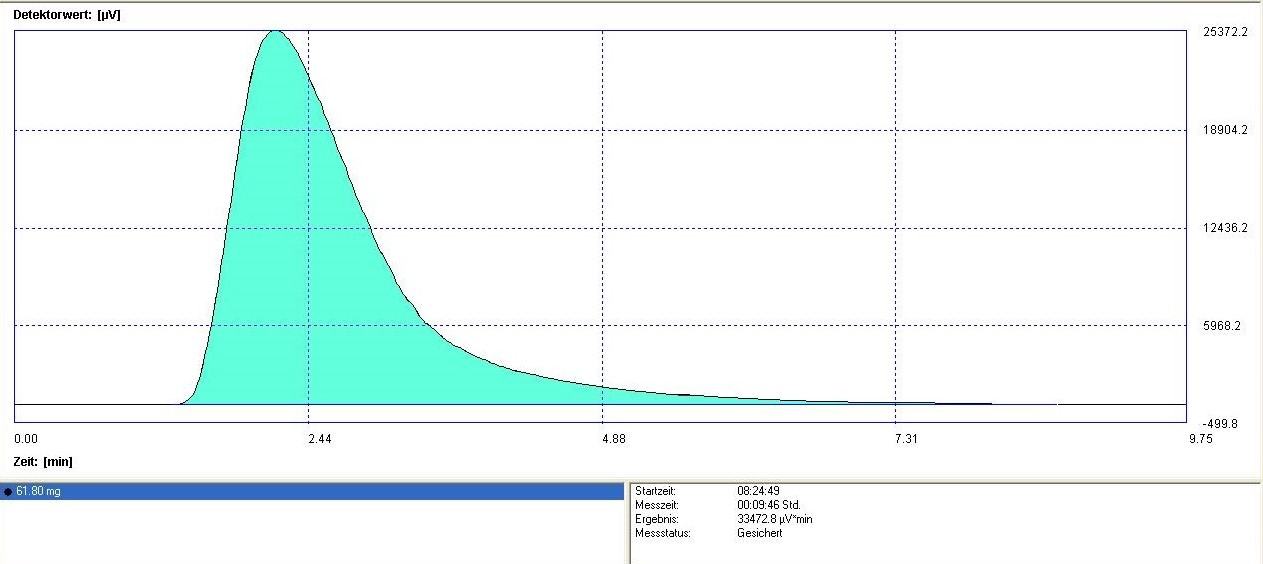
\includegraphics[width=0.75\textwidth]{img/CaCO3_k1}
	\caption{Messkurve 1 für Kalibrierung mit \ce{CaCO3}}
	\label{dia:k1}
\end{figure}
\FloatBarrier
%Ende

%Start
\begin{figure}[h!]
	\centering
	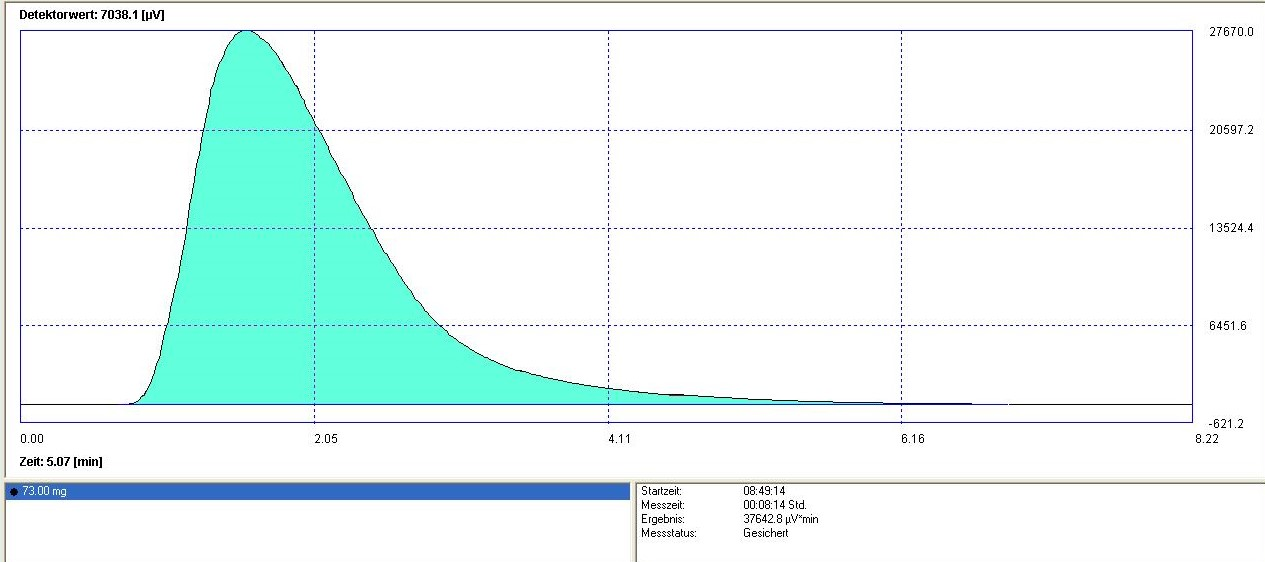
\includegraphics[width=0.75\textwidth]{img/CaCO3_k2}
	\caption{Messkurve 2 für Kalibrierung mit \ce{CaCO3}}
	\label{dia:k2}
\end{figure}
\FloatBarrier
%Ende

%Start
\begin{figure}[h!]
	\centering
	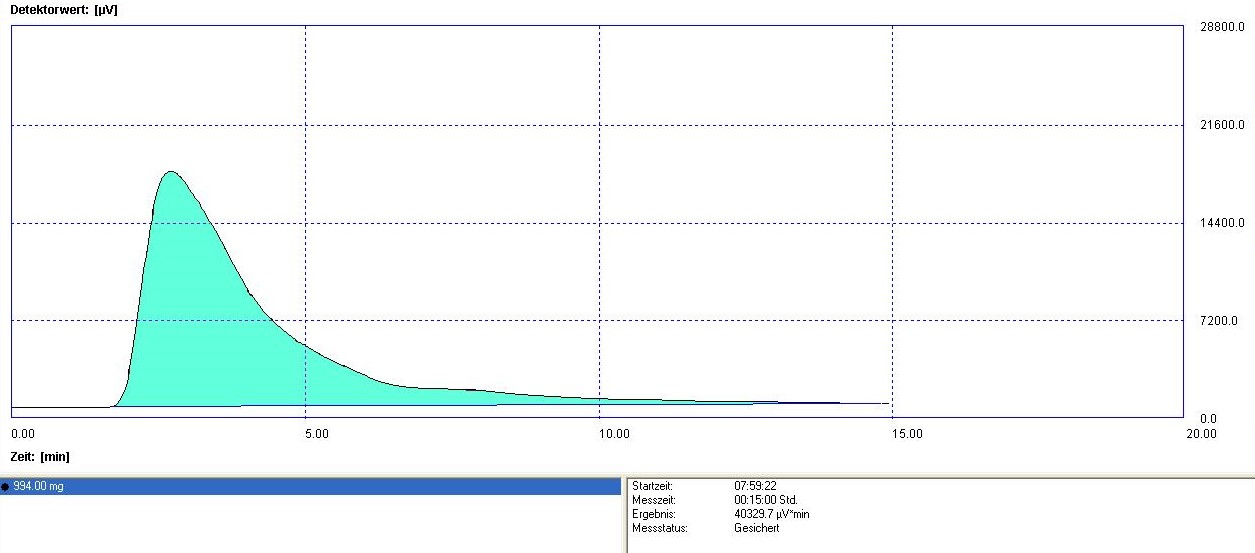
\includegraphics[width=0.75\textwidth]{img/Muell_V1}
	\caption{Messkurve für Müllprobe 1}
	\label{dia:m1}
\end{figure}
\FloatBarrier
%Ende

%Start
\begin{figure}[h!]
	\centering
	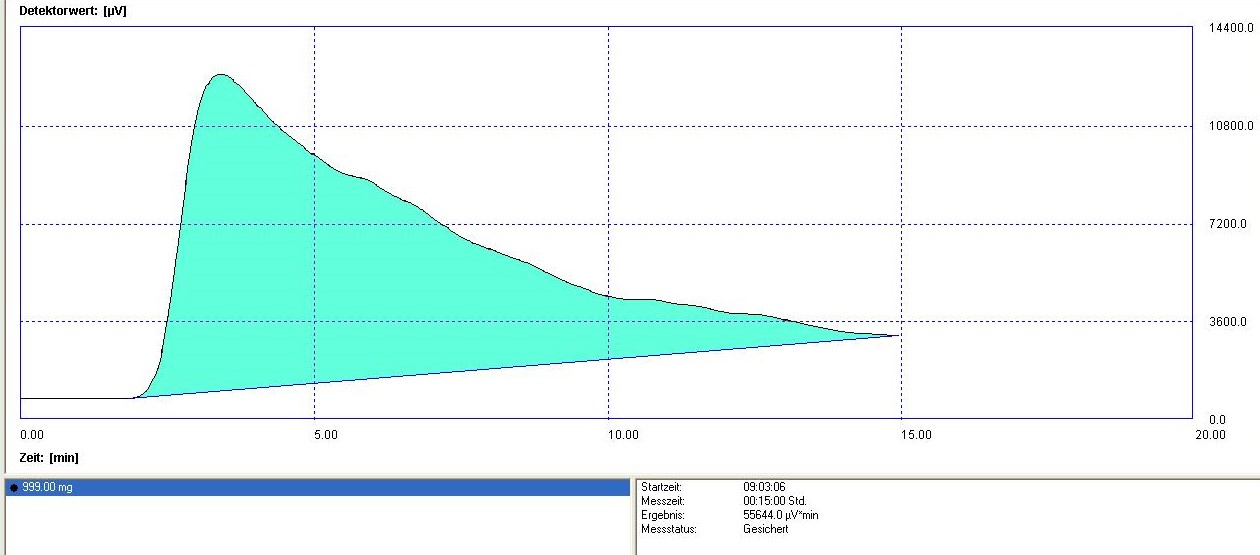
\includegraphics[width=0.75\textwidth]{img/Muell_V2}
	\caption{Messkurve für Müllprobe 2}
	\label{dia:m2}
\end{figure}
\FloatBarrier
%Ende

\newpage

Um die Messwerte im Vergleich zu den Blindproben beurteilen zu können sind diese im Diagramm \ref{dia:kalibrierkurve} aufgezeigt und werden mittels Abweichungsrechnung ab Gleichung \ref{gl:abweichung} weiter analysiert.

\begin{figure}[h!]
	\begin{center}
		\begin{tikzpicture}
		\begin{axis}[
		xlabel={$m_{Carbonat} \left[\si{\milli \gram}\right]$},
		ylabel={$\Phi \left[\si{\micro \volt \minute}\right]$},
		xmin = 0,
		xmax = 100,
		width= 15cm,
		height=6cm,
		ymin=0,
		ymax=70000,
		axis x line=bottom,
		axis y line=left,
		legend style={
			at={(0.2,-0.3)},anchor=north west}]
		
		\addplot [domain=0:200, samples=101,dotted]{902.97*x - 14.812};
		\addlegendentry{Verlauf der Messdaten $(902,97*x - 14,812)$};
		%\addplot [domain=0:200, samples=101,dashed]{476.91*x + 3876.1};
		\addplot [domain=0:200, samples=101,]{874.02*x + 141.53};
		\addlegendentry{Kalibrierkurve $(874,02*x + 141,53)$};
		\addplot+ [mark=*, color=black] coordinates {(44.68,40329.7)};
		\addlegendentry{\ce{CaCO3}-Müllprobe 1};
		\addplot [mark=*, color=black] coordinates {(61.64,55644.0)};
		\addlegendentry{\ce{CaCO3}-Müllprobe 2};
		\addplot [mark=x, color=blue, only marks] coordinates {(43.8,37642.8) (37.08,33472.8) (0,0)};
		\addlegendentry{\ce{CaCO3}-Blindproben};
		\end{axis}%
		\end{tikzpicture}%
	\end{center}
	\caption{Kalibrierkurve zur Bestimmung des Carbonatgehaltes der  Müllprobe II}
	\label{dia:kalibrierkurve}
\end{figure}
\FloatBarrier
\vspace*{-7mm}
\subsubsection{Abweichung von Kalibrierkurve}
\vspace*{-3mm}
\begin{flalign}
\label{gl:abweichung}
	a	&= \frac{\Phi_{Mess}-\Phi_{Kali}}{\Phi_{Kali}}\\[2mm]
	a_1	&= \frac{\SI{40329.7}{\micro \volt \minute}-\SI{39192.74}{\micro \volt \minute}}{\SI{39192.74}{\micro \volt \minute}} = \underline{\underline{2,9\%}}\\[2mm]
	a_2	&= \frac{\SI{55644.0}{\micro \volt \minute}-\SI{54016.12}{\micro \volt \minute}}{\SI{54016.12}{\micro \volt \minute}} = \underline{\underline{3,0\%}}
\end{flalign}

\newpage

\subsection{Bestimmung des TC}
\label{sec:tc}
Die Bestimmung des $TC$-Gehaltes erfolgt mittels \textit{Analysegerät} und ergibt einen Wert von \SI{274,26}{\gram \per \kg} der originalen Müllprobe II. Parallel erfolgte ebenfalls eine Bestimmung des $TC$s für eine Blindprobe mit Calciumcarbonat und der via $TIC$-Bestimmung vorbehandelten Probe. Die Messwerte für alle drei Proben sind in Tab. \ref{tab:tc_messung} aufgeführt.

\begin{figure}[h!]
	\renewcommand{\arraystretch}{1.2}
	\centering
	\caption{TC der Blindprobe, der originalen und der vorbehandelten Abfallprobe}
	\label{tab:tc_messung}
	\begin{tabular}{c|c|c}
		\hline
		\textbf{Probe} & \textbf{Probenmenge} & \textbf{Messwert}  \\
		\hline
		Blindprobe				&	\SI{234,3}{\milli \gram}	& \SI{0,41}{\mpercent}	\\
		Original				&	\SI{79,0}{\milli \gram}	& \SI{27,43}{\mpercent}		 \\
		Vorbehandelt mit TIC	&	\SI{474,9}{\milli \gram}	& \SI{4,39}{\mpercent}\\
		\hline
	\end{tabular}
\end{figure}
\FloatBarrier
\textcolor{red}{Diskussion: Blindprobe nicht 100\% Reinheit + Genauigkeit des Messgerätes}\\
\textcolor{red}{Diskussion: Plausibilität Vergleich (müsste Ok sein)}\\
\textcolor{red}{Diskussion: In wie fern Passt das mit TIC - müsste bei ca. 26\% liegen oder ?\\
Man könnte davon ausgehen, dass man damit den TOC Gehalt bestimmt hätte. Da ja aber NAOH und Phosphorsäure zugegeben wurde, ist die Masse der originalen Probe beeinflusst und der Wert mit 4,39\% nicht richtig. Man könnte zur Probe den Wert berechnen ohne NaOH und Phosphorsäure- ist mir zu aufwendig}

\subsection{Bestimmung des TOC}
An dieser Stelle wird ergänzend die Bestimmung des $TOC$ aufgezeigt.\linebreak
 Dies erfolgt via Berechnung der Differenzen des $TC$ und des $TIC$, \linebreak
dargestellt in den Gleichungen \ref{gl:1} bis \ref{gl:2}. 
Falls der $TOC$ für eine Auswertung wirklich relevant sollte, ist eine Bestimmung mittels einer extra Messmethode zu empfehlen, da durchaus in den Messungen des $TC$ oder des $TIC$ Fehler hätten auftreten können. Die hier aufgeführte, simple Methodik der $TOC$ Bestimmung könnte dann zur Plausibilitätsprüfung genutzt werden.
\begin{flalign}
\label{gl:1}
	TC	&= TIC+TOC\\
	TOC	&= TC-TIC \\
		&= \SI{27,43}{\mpercent}-\SI{1,1}{\mpercent}\\
		&= \underline{\underline{\SI{26,33}{\mpercent}\approx \SI{26}{\mpercent}}}
\label{gl:2}
\end{flalign}
\vspace*{-5mm}
\begin{figure}[h!]
	\renewcommand{\arraystretch}{1.2}
	\centering
	\caption{Daten zu den Kohlenstoffgehalten der originalen Abfallprobe II}
	\label{tab:kohlenstoffgehalte}
	\begin{tabular}{c|c|c||c}
		\hline
		\textbf{Kohlenstofftyp} & \textbf{Messwert} & \textbf{Berechnet} & \textbf{Approximiert}  \\
		\hline
		TC		&	\SI{27,43}{\mpercent}	& -							& $\approx \SI{27}{\mpercent}$ \\
		TIC		&	\SI{1,1}{\mpercent}		& -							& $\approx \SI{1}{\mpercent}$ \\
		TOC		&	-						& \SI{26,33}{\mpercent}		& $\approx \SI{26}{\mpercent}$\\
		\hline
	\end{tabular}
\end{figure}
\FloatBarrier

\textcolor{red}{Diskussion: TOC fehlt}

\newpage

\section{Bestimmung von Brenn- und Heizwert}
In diesem Abschnitt werden die Berechnungen und Ergebnisse zur Bestimmung der Trockensubstanz $TS$, des Wassergehaltes $W$, sowie des Glühverlustes $GV$ dargestellt. \\
Brenn- und Heizwert wurden mittels Näherungsformeln nach \textsc{Shin} bestimmt und geben Auskunft über die Wertigkeit der Müllprobe als Ersatzbrennstoff. Für die Berechnung wurden die Ergebnisse aus Tabelle \ref{tab:ts_w_gv} genutzt.

\subsubsection{Bestimmung des Trockensubstanzgehalt $\mathbf{TS}$} 
\begin{flalign}
TS \left[\%\right]	&= \frac{m_{\text{Trockensubstanz}}}{m_\text{gesamt}}*100\%\\
TS_{\text{TIC}}		&= \frac{\SI{7,340}{\gram}}{\SI{38,717}{\gram}}*100\%\\
&=\underline{18,96\%}\\[2mm]
TS_{\text{org.}}		&= \frac{\SI{2,878}{\gram}}{\SI{2,976}{\gram}}*100\%\\
&=\underline{96,71\%}
\end{flalign}

\subsubsection{Bestimmung des Wassergehaltes $\mathbf{W}$} 
%Trockensubstanz TIC = 38,717 dann 7,340
%TS original = 2,976 dann 2,878
\begin{flalign}
W \left[\%\right]	&= \frac{m_\text{gesamt}-m_{\text{Trockensubstanz}}}{m_\text{gesamt}}*100\%\\
W_{\text{TIC}}		&= \frac{\SI{38,717}{\gram}-\SI{7,340}{\gram}}{\SI{38,717}{\gram}}*100\%\\
&=\underline{81,04\%}\\[2mm]
W_{\text{org.}}		&= \frac{\SI{2,976}{\gram}-\SI{2,878}{\gram}}{\SI{2,976}{\gram}}*100\%\\
&=\underline{3,29\%}
\end{flalign}

\subsubsection{Bestimmung des Glühverlustes $\mathbf{GV}$}
%VERBENNUNG
\begin{flalign}
GV \left[\%\right]				&= \frac{m_{\text{gesamt}}-m_{\text{Glührückstand}}}{m_\text{gesamt}}*100\%\\[2mm]
GV_{\text{org.}} &= \frac{\SI{2,878}{\gram}-\SI{2,203}{\gram} }{\SI{2,878}{\gram}}*100\%\\
&= \underline{\SI{23,45}{\percent}}
\end{flalign}

\subsubsection{Bestimmung des Inertstoffgehaltes $\boldsymbol{IS}$}
%VERBENNUNG
\begin{flalign}
IS\left[\%\right]				&= \SI{100}{\percent}-TC-W\\
IS_{\text{org.}} &\approx \SI{100}{\percent}-\SI{25}{\percent}-\SI{3}{\percent}\\
&\approx \underline{\SI{72}{\percent}}
\end{flalign}

%Tabelle START
\vspace*{-.5cm}
\renewcommand{\arraystretch}{1.2}
\begin{table}[h!]
	\centering
	\caption{Daten zu Trockensubstanz, Wassergehalt, Glühverlust und \mbox{Inertstoffgehalt} \\ der Müllprobe II}
	\label{tab:ts_w_gv}
	%\resizebox{10cm}{!}{
	\begin{tabulary}{1.2\textwidth}{C|CC|CC}
		\hline
		\textbf{Probe} & \textbf{Trockensubstanz} & \textbf{Wassergehalt} & \textbf{Glühverlust} & \textbf{Inertstoffgehalt}\\ 
		\hline
		Original & 96,71\% & 3,29\% & 23,45\%&76,55\%\\
		Nach TIC & 18,96\% & 81,04\% & - & -\\
		\hline
	\end{tabulary}
	%}
\end{table}
\FloatBarrier
\vspace*{-2.5mm}
%Tabelle Ende

\subsubsection{Bestimmung des Brennwertes $\mathbf{H_s}$}
\begin{flalign}
	H_s \left[\si{\kilo \joule \per \kg}\right]		&= 523*GV^{0,77}\\
	H_s(org.)	&= 523*23,45^{0,77}\\	
				&= \underline{\underline{\SI{5936,24}{\kilo \joule \per \kg}\approx\SI{5,94}{\mega \joule \per \kg}\approx\SI{1,65}{\kWh \per \kg}}}
\end{flalign}


\subsubsection{Bestimmung des Heizwertes $\mathbf{H_i}$} 
\begin{flalign}
H_i	\left[\si{\kilo \joule \per \kg}\right]	&= H_s*\frac{TS}{100}-25*\left(0,09*H*TS+W\right)\\
											&= H_s*\frac{TS}{100}-25*\left(0,09*\frac{GV}{15}*TS+W\right)\\[2mm]
H_i(org.)		&= \SI{5936,24}{\kilo \joule \per \kg}*\frac{96,71}{100}-25*\left(0,09*\frac{23,45}{15}*96,71+3,29\right)\\
				&= \underline{\underline{\SI{5318,51}{\kilo \joule \per \kg}\approx\SI{5,32}{\mega \joule \per \kg}\approx\SI{1.48}{\kWh \per \kg}}}
\end{flalign}
 
